\documentclass[tikz, border=10pt]{standalone}
\usepackage{tikz}
\usepackage{amsmath}
\usetikzlibrary{calc}

\begin{document}
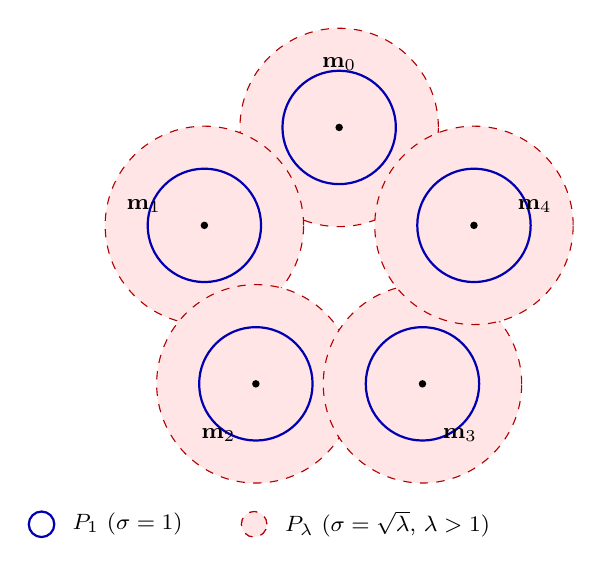
\begin{tikzpicture}[font=\sffamily, scale=0.9]

    % K = 5 class means on a regular K-gon of radius r = 2. mu_0 sits
    % at the top (angle 90 deg); the remaining four vertices are spaced
    % 72 deg apart going counter-clockwise.
    \def\sep{2}
    \def\sigP{0.8}
    \def\sigQ{1.4}

    % Q variance contours, drawn first so the P0 rings sit on top.
    \foreach \i in {0,1,2,3,4} {
        \pgfmathsetmacro{\angle}{90 + 72 * \i}
        \pgfmathsetmacro{\xc}{\sep*cos(\angle)}
        \pgfmathsetmacro{\yc}{\sep*sin(\angle)}
        \fill[red!10] (\xc,\yc) circle (\sigQ);
        \draw[red!70!black, dashed, thin] (\xc,\yc) circle (\sigQ);
    }

    % P0 variance contours plus class-mean dots.
    \foreach \i in {0,1,2,3,4} {
        \pgfmathsetmacro{\angle}{90 + 72 * \i}
        \pgfmathsetmacro{\xc}{\sep*cos(\angle)}
        \pgfmathsetmacro{\yc}{\sep*sin(\angle)}
        \draw[blue!70!black, thick] (\xc,\yc) circle (\sigP);
        \fill[black] (\xc,\yc) circle (1.5pt);
        \pgfmathsetmacro{\lxc}{1.45*\xc}
        \pgfmathsetmacro{\lyc}{1.45*\yc}
        \node[font=\footnotesize] at (\lxc,\lyc) {$\mathbf{m}_{\i}$};
    }

    % Legend.
    \begin{scope}[shift={(-4.2, -3.6)}, font=\footnotesize]
        \draw[blue!70!black, thick] (0,0) circle (0.18);
        \node[anchor=west] at (0.3, 0) {$\mathbb{P}_1$ ($\sigma = 1$)};
        \draw[red!70!black, dashed, thin] (3.0, 0) circle (0.18);
        \fill[red!10] (3.0, 0) circle (0.18);
        \draw[red!70!black, dashed, thin] (3.0, 0) circle (0.18);
        \node[anchor=west] at (3.3, 0) {$\mathbb{P}_\lambda$ ($\sigma = \sqrt{\lambda}$, $\lambda > 1$)};
    \end{scope}

\end{tikzpicture}
\end{document}
